\chapter{Introduction}\label{ch:introduction}
		Application	Software is program or group of program customised to perform group of activities for end user. Generally software are classified as system software and application software.System software consists of low-level programs that is designed to run computer's hardware and application programs like compilers, loaders, linkers and so on. Application software resides above system software like database programs, word processors, spreadsheets. In this survey, we focus on the architecture and process involved in development of different types of application software. 

		Software application architecture is the process of designing a structured solution that focuses on how the components in the applications interact with each other, while optimizing common quality attributes such as performance, security, and manageability.The architecture are structured with consideration of user and the business goals.The selection of data structures and algorithms are design concerns which would overlap with architecture concerns.These scenarios where the both of them overlap are discussed in detailed in later chapters.The architecture must be flexible to handle the changes in software or hardware technologies and requirements that are not known in the early stages of design process as the design of the application will evolve during the development stages.
			
	
\section{Command-Line Application}
			
			Technology has come long way since the first computers were created, back around the start of World War II. The first generation of software application are command line programs which are mostly single command at a time and uses it to accomplish all the application requirements in that particular loop. These programs are shared as binaries(executables) which can be compiled from the source code, specific to the architecture. 

\section{Desktop Application}
			
			In spite of early application which was designed to run from mainframe computers and accessed through terminals devices, the proposal of powerful desktop applications which can be run in the local personal computer dethroned the previous generation application software. The mainframe was replaced with server by the client server model which induced distributed application structure that partitions tasks or workload between the service provider (Server) and the service requester (Client).  
			
\section{Web Application}
			
			Steady enhancements in hardware specifications and broadband speeds led to major improvements in the quality and quantity of WWW content. Websites inflated their features beyond static web pages by becoming more interactive with the increase of multimedia content. As browsers and development platforms evolved, and more and more people began to use the internet and email, more businesses established their presence in the online world. These businesses leveraged the emerging interactive capabilities of the web to introduce applications that were served directly to a web browser, and these web applications became very popular.

\section{Mobile Application}
			
			Nowadays, an ever-growing percentage of portable device like smart phones have doubled the number of users accessing the internet  on their smart phones.The need of mobile applications became pretty obvious. Mobile applications should be designed in such a way that the power consumption and processing power is reduced. Android and iOS being the major players in the industry, they natively support java and ObjectiveC as the native language. 
			
			The mobile applications can be categorised into mobile web application, native application and hybrid application.A native application is developed for a certain mobile device (smart phone, tablet, so on). They’re installed directly onto the device. Users typically acquire these applications through an online store or marketplace such as The App Store or Android Apps on Google Play.It was started working as standalone, and in the recent years, we see a lot of integration with the web which is named as hybrid application.


\begin{figure}[!htb]	
  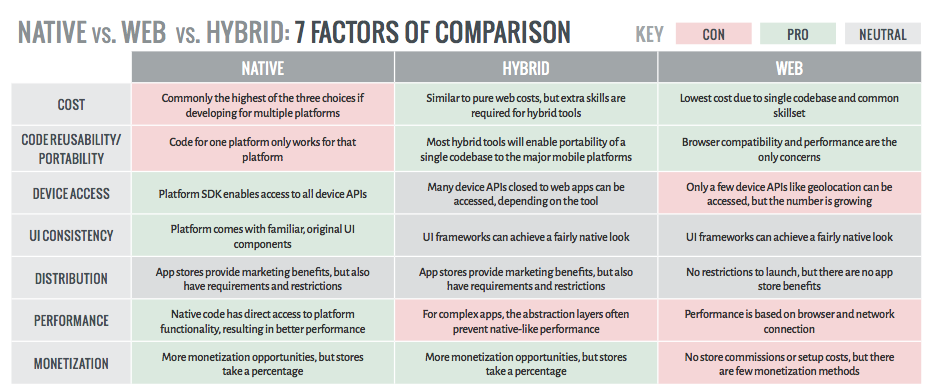
\includegraphics[max width=\linewidth,scale = 3]{figures/MobAppTypes.png}
	 \caption{Native vs Web vs Hybrid}
  \label{fig: Native vs Web vs Hybrid}
\end{figure}	
			
			 Internet-enabled applications that have specific functionality for mobile devices are called as mobile web application. They are accessed through the mobile device’s web browser (i.e. on the iPhone, this is Safari by default) and they don’t need to be downloaded and installed on the device.Although mobile websites and mobile apps aren't the same thing, they generally offer the same features that can help grow business by making it easier for customers to find and reach it. 
			

%\section{Desktop Application}
%You can also have examples in your document such as in example~\ref{ex:simple_example}.
%\begin{example}{An Example of an Example}
%  \label{ex:simple_example}
%  Here is an example with some math
%  \begin{equation}
%    0 = \exp(i\pi)+1\ .
%  \end{equation}
%  You can adjust the colour and the line width in the {\tt macros.tex} file.
%\end{example}
%
%\section{Web Application}
%Well, like this
%\subsection{This is a Subsection}
%and this
%\subsubsection{This is a Subsubsection}
%and this.
%
%\paragraph{A Paragraph}
%You can also use paragraph titles which look like this.
%
%\subparagraph{A Subparagraph} Moreover, you can also use subparagraph titles which look like this\todo{Is it possible to add a subsubparagraph?}. They have a small indentation as opposed to the paragraph titles.
%
%\todo[inline,color=green]{I think that a summary of this exciting chapter should be added.}
%
%\section{Mobile Application}
%Well, like this
%\subsection{This is a Subsection}
%and this
%\subsubsection{This is a Subsubsection}
%and this.
%
%\paragraph{A Paragraph}
%You can also use paragraph titles which look like this.
%
%\subparagraph{A Subparagraph} Moreover, you can also use subparagraph titles which look like this\todo{Is it possible to add a subsubparagraph?}. They have a small indentation as opposed to the paragraph titles.
%
%\todo[inline,color=green]{I think that a summary of this exciting chapter should be added.}